\chapter{Lösungskonzept}

Das Lösungskonzept beinhaltet die Grundlagen für die erfolgreiche Umsetzung des Prototypen. Der Inhalt ist hauptsächlich aus den Bereich Management und Anforderungen. Die unter Anforderungen aufgenommenen Punkte sind in Zusammenarbeit mit dem Projektpartner entstanden, um so auch die Ansprüche des Forschungsprojektes zu erfüllen.

\section{Projektmanagement}

Führung und Kontrolle des Projekte werden im folgenden Kapitel aufgezeigt. Das Management funktioniert agil, dafür werden geeignete Methoden (vgl. \textit{ScrumDo}) eingesetzt.

\subsection{Projektstrukturplan}
Die \autoref{fig:projektstrukturplan} gewährt einen Überblick über das Projekt. Sie stellt die wichtigsten Bereich und Phasen dar, worin die Arbeit grob eingegliedert werden kann.

\begin{figure}[ht]
\centering
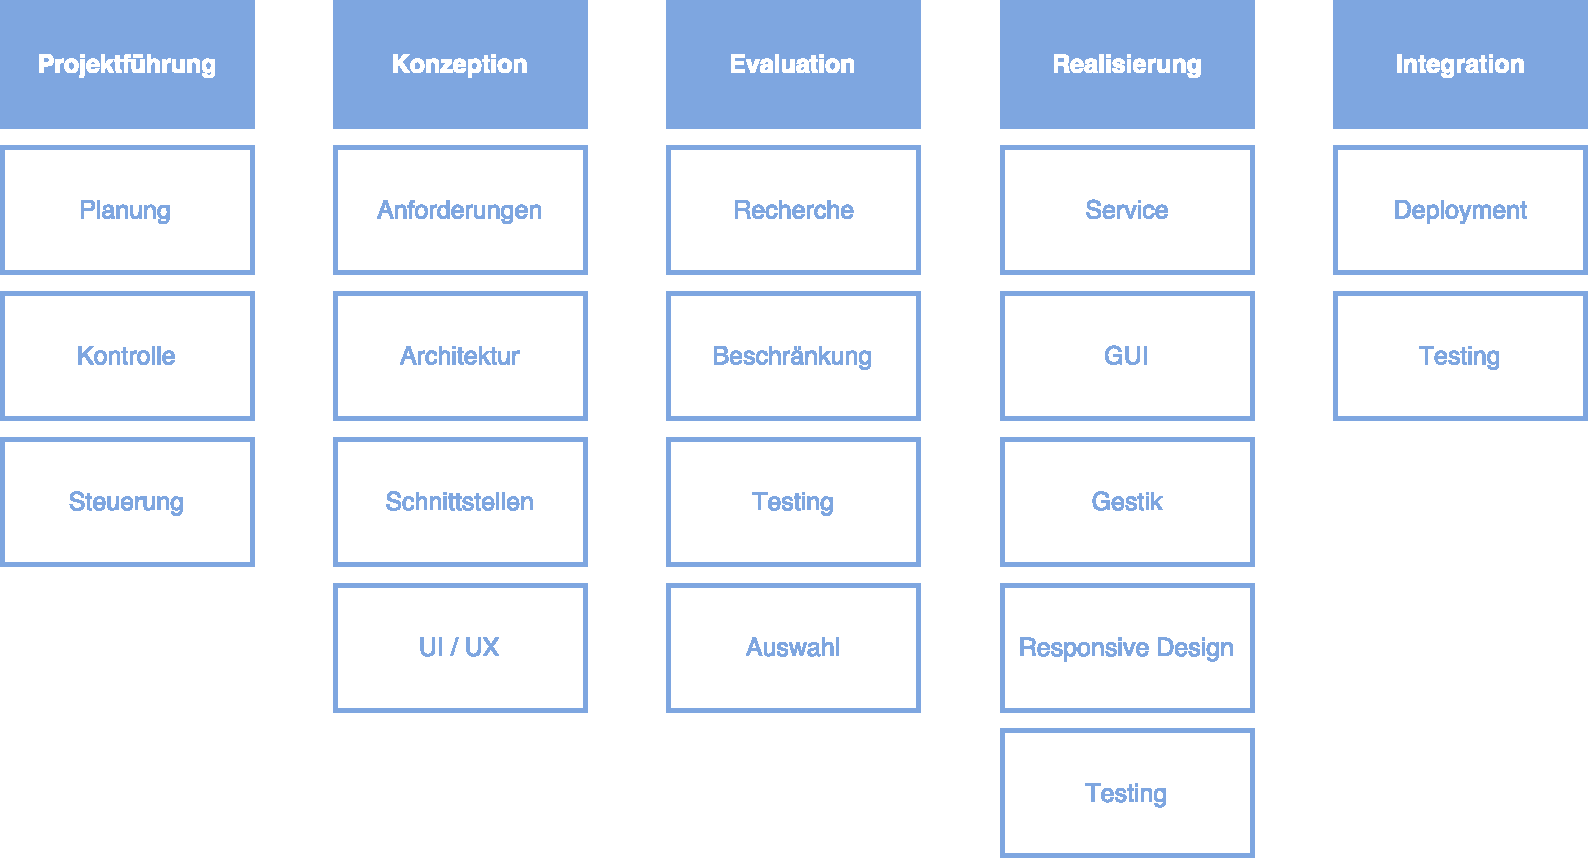
\includegraphics[width=0.7\textwidth]{Projektstrukturplan}
\caption{Projektstrukturplan}
\label{fig:projektstrukturplan}
\end{figure}


\subsection{Projektführung}



\section{Anforderungen}

Für die weitere Unterteilung in Arbeitspakete und Stories, werden die Anforderungen zunächst in Prosa gesammelt. Diese entstammen dem Kundenworkshop und der Aufgabenstellung.

\subsection{Projektmanagement}

\begin{enumerate}
    \item Das Projekt wird agil in allen Bereichen agil geführt.
\end{enumerate}

\subsection{Funktionale Anforderungen}

\begin{table}
  \centering
  \begin{tabular}{|p{0.6cm} | p{1.6cm} | p{8cm}|}
  \hline
    ID & Priorität & Beschreibung \\\hline
    A1 & X & Die zugrunde liegende Datenbasis kann mittels eines Graphen visualisiert werden. Jener besteht aus Knoten und Kanten, welche gerichtet und beschriftet sind.\\\hline
    A2 & X & Der zu erarbeitende Prototyp kann bidirektional mit dem \textit{ikc-core}-Prototypen interagieren. Änderungen am \textit{ikc-core} sind in der Visualisierung sichtbar. Es ist jedoch es auch möglich Änderungen direkt in der Visualisierung vorzunehmen.\\\hline
    A3 & X & Mittels der Visualisierung können die grundlegenden Datenbankoperationen \textit{CREATE}, \textit{READ}, \textit{UPDATE} und \textit{DELETE} (CRUD) direkt auf der Datenbasis des \textit{ikc-core} angewendet werden.\\\hline
    A4 & X & Der Prototyp kann auf Smartphones und Tablets benutzt werden.\\\hline
    A5 & X & Der Prototyp kann auf Laptops und Desktop-Computern benutzt werden.\\\hline    
    A6 & X & Mit Hilfe verschiedener Kriterien (beispielsweise Kontext oder Nachbarschaft) kann ein Teilgraph visualisiert werden.\\\hline 
    A7 & X & Die Visualisierung kann in verschiedenen Projekten wiederverwendet werden.\\\hline     
     
  \end{tabular}
    \caption{Funktionale Anforderungen}
  \label{tab:funktionale-anforderungen}
\end{table}

\begin{enumerate}
    \item Die zugrunde liegende Datenbasis kann mittels eines Graphen visualisiert werden. Jener besteht aus Knoten und Kanten, welche gerichtet und beschriftet sind.
    \item Der zu erarbeitende Prototyp kann bidirektional mit dem \textit{ikc-core}-Prototypen interagieren. Änderungen am \textit{ikc-core} sind in der Visualisierung sichtbar. Es ist jedoch es auch möglich Änderungen direkt in der Visualisierung vorzunehmen.
    \item Mittels der Visualisierung können die grundlegenden Datenbankoperationen \textit{CREATE}, \textit{READ}, \textit{UPDATE} und \textit{DELETE} (CRUD) direkt auf der Datenbasis des \textit{ikc-core} angewendet werden.
    \item Die Entwicklung erfolgt nach dem Ansatz \textit{mobile-first}, was bedeutet, dass absteigend nach der Priorität die Darstellung für die folgenden Plattformen, Mobile, Tablet, Laptop und Desktop, entwickelt wird.
    \item Der Prototyp kann auf Smartphones und Tablets benutzt werden.
    \item Der Prototyp kann auf Laptops und Desktop-Computern benutzt werden.
    \item Mit Hilfe verschiedener Kriterien (beispielsweise Kontext oder Nachbarschaft) kann ein Teilgraph visualisiert werden.
    \item Die Visualisierung kann in verschiedenen Projekten wiederverwendet werden.
\end{enumerate}

\subsection{Nicht funktionale Anforderungen}

\begin{table}
  \centering
  \begin{tabular}{|p{0.4cm} | p{1.3cm} | p{8cm}|}
  \hline
     ID & Priorität & Beschreibung \\\hline
     1 & X & Die zugrunde liegende Datenbasis kann mittels eines Graphen visualisiert werden. Jener besteht aus Knoten und Kanten, welche gerichtet und beschriftet sind.\\\hline
     2 & X & Die zugrunde liegende Datenbasis kann mittels eines Graphen visualisiert werden. Jener besteht aus Knoten und Kanten, welche gerichtet und beschriftet sind.\\\hline
     
  \end{tabular}
    \caption{Nicht funktionale Anforderungen}
  \label{tab:nicht-funktionale-anforderungen}
\end{table}

\begin{enumerate}
    \item Die Visualisierung kann direkt nahtlos innerhalb des \textit{ikc-core} verwendet werden.
    \item Bestehende Funktionen (beispielsweise \textit{New Node}, \ldots) können teilweise direkt in der Visualisierung dargestellt werden.
    \item Der zu entwicklende Prototyp kann zur Verfügung stehende Schnittstellen des \textit{ikc-core} verwenden.
    \item Der Prototyp kann (unter anderem) mit Drag and Drop bedient werden.
\end{enumerate}


\section{Stories}

\begin{table}
  \centering
  \caption{Things you (usually) don't say}
  \label{tab:things-you-dont-say}
  \begin{tabular}{lll}
    \toprule
    \st{It holds (that) \dots} & We have \dots & \emph{Es gilt \dots}\\
    \multicolumn{3}{l}{\quad\footnotesize(`Equation (5) holds.' is fine, though.)}\\
    \st{$x$ fulfills property $\mathcal{P}$.}& \(x\) satisfies property \(\mathcal{P}\). & \emph{\(x\) erfüllt Eigenschaft \(\mathcal{P}\).} \\
    \st{in average} & on average & \emph{im Durchschnitt}\\
    \st{estimation} & estimate   & \emph{Abschätzung}\\
    \st{composed number} & composite number & \emph{zusammengesetzte Zahl}\\
    \st{with the help of} & using & \emph{mit Hilfe von}\\
    \st{surely} & clearly & \emph{sicher, bestimmt}\\
    \st{monotonously increasing} & monotonically incr. & \emph{monoton steigend}\\
    \multicolumn{3}{l}{\quad\footnotesize(Actually, in most cases `increasing' is just fine.)}\\
    \bottomrule
  \end{tabular}
\end{table}
